\chapter{Cenni teorici}

In questo capitolo, verrà fornita un'introduzione approfondita agli standard e alle tecnologie che sono stati considerati nell'ambito della nostra attività. La comprensione di tali standard è fondamentale per contestualizzare le scelte progettuali e le strategie implementate. Ci concentreremo su diversi protocolli e specifiche tecniche che hanno influenzato lo sviluppo delle soluzioni adottate, esplorando le loro caratteristiche distintive, le modalità di funzionamento e le applicazioni pratiche.

In particolare, analizzeremo gli standard relativi alla comunicazione wireless nell'ambito \textit{automotive}, come WAVE (\textit{Wireless Access in Vehicular Environments}), che gioca un ruolo cruciale nella connettività dei veicoli e nella gestione delle reti di trasporto intelligenti. 

Successivamente, esamineremo il meccanismo EDCA (\textit{Enhanced Distributed Channel Access}), che è una parte integrante del livello MAC (\textit{Media Access Control}) nel contesto delle reti wireless. EDCA introduce un metodo di accesso al canale più sofisticato rispetto al tradizionale DCF (\textit{Distributed Coordination Function}), permettendo una gestione più efficiente delle priorità di traffico. Questo è particolarmente importante in scenari in cui coesistono diversi tipi di traffico, come video, voce e dati, ognuno con requisiti di latenza e larghezza di banda diversi. Discuteremo come EDCA assegna diverse code di accesso per garantire che le comunicazioni più critiche ricevano la priorità necessaria, migliorando così l'esperienza complessiva degli utenti.

Attraverso questa analisi di WAVE e EDCA, il capitolo intende fornire una comprensione approfondita delle tecnologie che supportano le comunicazioni nei veicoli connessi, evidenziando come queste innovazioni possano contribuire a una mobilità più sicura ed efficiente.

%\section{ITS - Intelligent Transport System}

%\section{VANET}

\section{IEEE WAVE}
WAVE è progettato specificamente per ambienti di trasporto, consentendo la comunicazione tra veicoli (\textit{V2V: Vehicle-to-Vehicle}) e tra veicoli e infrastrutture stradali (\textit{V2I: Vehicle-to-Infrastructure}). Questo protocollo sfrutta canali wireless dedicati per garantire una bassa latenza e una maggiore affidabilità, elementi essenziali per applicazioni critiche come la prevenzione degli incidenti e la gestione del traffico. 

Per facilitare questo, l'IEEE ha introdotto un emendamento specifico al protocollo 802.11, noto come 802.11p\cite{std2007wireless}. Questo emendamento si occupa sia del livello fisico, chiamato PHY, sia della gestione dell'accesso al canale, che riguarda il livello MAC. Non ci soffermeremo ulteriormente sui livelli superiori, se non attraverso un breve excursus, poiché il protocollo in questione supporta senza difficoltà qualsiasi tipo di livello, sia esso basato su IP o meno\cite{DSRC-Based-vehicular}. Degno di nota è il fatto che è stato previsto un apposito protocollo per l'invio di frame che non richiedono un livello di trasporto come TCP o UDP, denominato \textit{WAVE Short Message Protocol (WSMP)}.

\begin{figure}[h!]
    \centering
    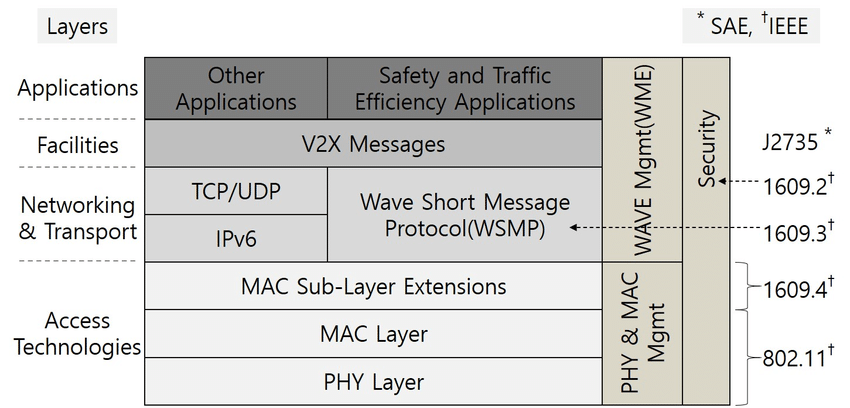
\includegraphics[width=0.7\textwidth]{WAVE-protocol-stack.png}
    \caption{Stack protocollo WAVE}
    \label{fig:wave_stack}
\end{figure}

Di seguito, presentiamo un elenco che fornisce ulteriori dettagli sui protocolli menzionati nella Figura \ref{fig:wave_stack}, partendo dal layer fisico e salendo di volta in volta:

\begin{itemize}
    \item \textit{IEEE 802.11-2016, IEEE Std 802.11p: Wireless Access in Vehicular Environments}.
    \item \textit{IEEE 1609.0: IEEE Guide for Wireless Access in Vehicular Environments (WAVE) Architecture}, con le sue varie componenti\cite{8686445}: 
        \begin{itemize}
            \item \textit{IEEE 1609.4: IEEE Standard for Wireless Access in Vehicular Environments (WAVE) - Multi-Channel Operation}; per il \textit{channel routing} e il \textit{channel coordination}\cite{7435228}.
            \item \textit{IEEE 1609.3: IEEE Standard for Wireless Access in Vehicular Environments (WAVE) - Networking Services}; per i sopracitati \textit{WAVE Short Messages}\cite{9374154}.
            \item \textit{IEEE 1609.2: IEEE Standard for Wireless Access in Vehicular Environments - Security Services for Applications and Management Messages}; per tutti gli aspetti relativi alla sicurezza\cite{10075082}.
        \end{itemize}
\end{itemize}

Risultano, anche, essere presenti altre varie componenti del protocollo \textit{IEEE 1609.0} su cui non ci si soffermerà e si riportano per completezza:

\begin{itemize}
    \item \textit{IEEE 1609.11:  IEEE Standard for Wireless Access in Vehicular Environments (WAVE) - Over-the-Air Electronic Payment Data}; standard per i pagamenti elettronici in applicazione \textit{WAVE based}\cite{5692959}.
    \item \textit{IEEE 1609.12:  IEEE Standard for Wireless Access in Vehicular Environments (WAVE) - Identifier Allocations}; standard per l'allocazione degli identificatori \textit{WAVE}\cite{8877516}.
\end{itemize}

Per concludere, alla luce del fatto che il contesto preso in esame, quello veicolare, richiede uno scambio di informazioni con latenze minime, \textit{WAVE} si basa interamente su una nuova modalità Wireless, simile alla classica \textit{ad hoc}, chiamata \textit{OCB (Outside Context of a Basic Service Set)}. Questo è un approccio che consente la trasmissione di dati al di fuori delle limitazioni tradizionali delle reti Wi-Fi, permettendo una comunicazione più flessibile e diretta tra i dispositivi, senza la necessità di passare attraverso infrastrutture quali i punti di accesso (\textit{Access Point}).

\subsection[Layer fisico]{Layer fisico}
L'IEEE 802.11p è uno standard della famiglia IEEE 802.11 progettato specificamente per la comunicazione wireless in ambienti vehicolari. È una tecnologia di rete che consente la comunicazione tra veicoli e tra veicoli e infrastrutture, facilitando applicazioni come la sicurezza stradale, la gestione del traffico e i servizi di infotainment.

Esso, innanzitutto, è basato su una modulazione OFDM (\textit{Orthogonal Frequencies Division Multiplexing}), ove in un totale di 64 sottoportanti, 48 vengono utilizzate per la trasmissione delle informazioni e 4 sono pilota; supporta velocità differenti in base alla modulazione delle sottoportanti e alla larghezza di banda utilizzati.

Di seguito una tabella riassuntiva dei parametri appena citati, suddivisi per \textit{bandwidth}:

\clearpage % Forza la stampa delle tabelle e figure in sospeso

\begin{table}[htbp]
    \centering
    \begin{tabular}{|p{7em}|p{7em}|p{7em}|p{7em}|} 
     \hline
     \textbf{Parametri} & \textbf{20 MHz} & \textbf{10 MHz} & \textbf{5 MHz} \\ 
     \hline
     \textbf{Bit rate (Mbit/s)} & 6, 9, 12, 18, 24, 36, 48, 54 & 3, 4.5, 6, 9, 12, 18, 24, 27 & 1.5, 2.25, 3, 4.5, 6, 9, 12, 13.5 \\ 
     \hline
     \textbf{Modulation} & BPSK, QPSK, 16/64QAM & BPSK, QPSK, 16/64QAM & BPSK, QPSK, 16/64QAM \\
     \hline
     \textbf{Code rate} & 1/2, 2/3, 3/4 & 1/2, 2/3, 3/4 & 1/2, 2/3, 3/4 \\
     \hline
     \textbf{Subcarriers} & 52 & 52 & 52 \\
     \hline
     \textbf{Spacing} & 312.5 kHz & 156.25 kHz & 78.125 kHz \\ 
     \hline
    \end{tabular}
    \caption{Parametri delle diverse larghezze di banda}
    \label{table:1}
\end{table}

Parlando circa le frequenze utilizzate, l'IEEE 802.11p opera nella banda di frequenza di 5,9 GHz (5,850 - 5,925 GHz), con le larghezze di canale citate nella Tabella \ref{table:1}. Questo standard consente l'uso di circa 9 canali, come illustrato nella Figura \ref{fig:frequency}. Tra questi, i canali 172 (5.860 GHz) e 184 (5.920 GHz) sono dedicati alla sicurezza: il primo fornisce una soluzione robusta per la sicurezza, mentre il secondo funge da protezione contro la congestione su altri canali\cite{ad_hoc_new}.

\begin{figure}[h!]
    \centering
    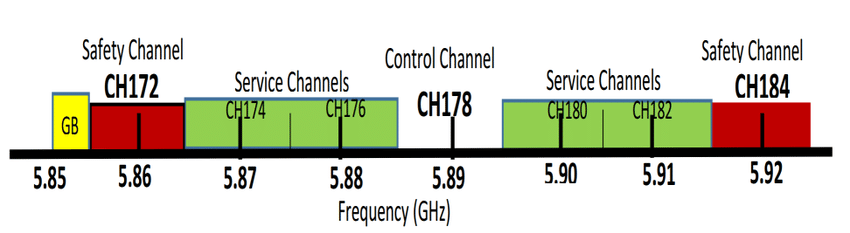
\includegraphics[width=0.7\textwidth]{frequency.png}
    \caption{Frequenze dell'IEEE 802.11p}
    \label{fig:frequency}
\end{figure}

Il canale 178 (5.890 GHz) è un canale di controllo, responsabile della gestione della trasmissione e della creazione del collegamento. Inoltre, sono disponibili sei canali di servizio per la comunicazione bidirezionale tra diversi tipi di unità.

\subsection[Layer MAC]{Layer MAC}

\section[EDCA]{EDCA}

\subsection[IEEE 1609.4 for multi-channel operations]{IEEE 1609.4 for multi-channel operations}